%\begin{figure}[hbt]
%  \centering
%  \label{fig:}
%  \subfigure[CAP]{
%    \includegraphics[width=0.4\textwidth]{}
%  }
%  \caption{}
%\end{figure}
\newcolumntype{S}{>{\centering\arraybackslash} m{0.26\textwidth} }

~\vfill

\begin{figure}[hbt]
	\centering
	\label{fig:errors}
	\subfigure[Haar $@$ 50 Error]{
		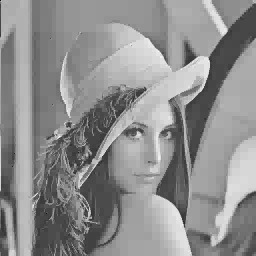
\includegraphics[height=0.25\textwidth]{../images/lenna_d2_50}
	}
	\subfigure[Haar $@$ 100 Error]{
		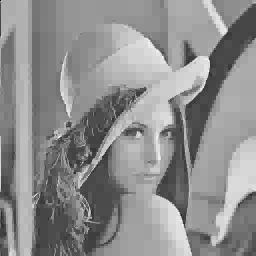
\includegraphics[height=0.25\textwidth]{../images/lenna_d2_100}
	}
	\subfigure[Haar $@$ 400 Error]{
		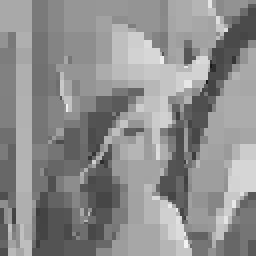
\includegraphics[height=0.25\textwidth]{../images/lenna_d2_400}
	} \\
	\subfigure[D-4 $@$ 50 Error]{
		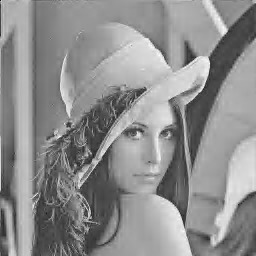
\includegraphics[height=0.25\textwidth]{../images/lenna_d4_50}
	}
	\subfigure[D-4 $@$ 100 Error]{
		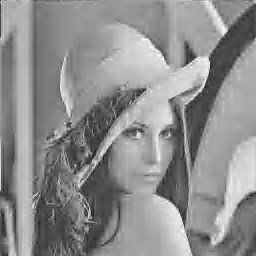
\includegraphics[height=0.25\textwidth]{../images/lenna_d4_100}
	}
	\subfigure[D-4 $@$ 400 Error]{
		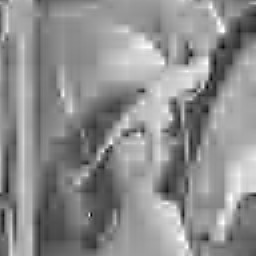
\includegraphics[height=0.25\textwidth]{../images/lenna_d4_400}
	} \\
	\subfigure[D-20 $@$ 50 Error]{
		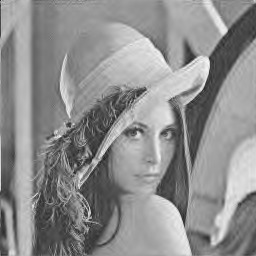
\includegraphics[height=0.25\textwidth]{../images/lenna_d20_50}
	}
	\subfigure[D-20 $@$ 100 Error]{
		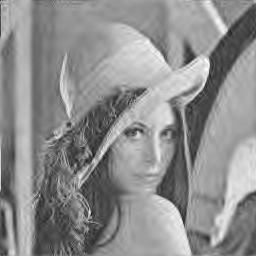
\includegraphics[height=0.25\textwidth]{../images/lenna_d20_100}
	}
	\subfigure[D-20 $@$ 400 Error]{
		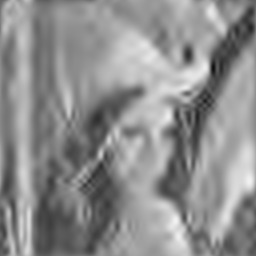
\includegraphics[height=0.25\textwidth]{../images/lenna_d20_400}
	} \\
	\caption{Results of different wavelets with different amounts of reconstruction error. The mean square error forumla was used to calculate error.}
\end{figure}

\vfill

~\vfill

\begin{figure}[hbt]
	\centering
	\label{fig:lenna_imgs}
	\begin{tabular}{ S @{} S @{} S }
		\centering
		& 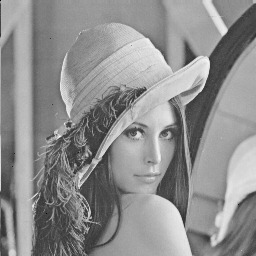
\includegraphics[height=0.25\textwidth]{../images/lenna} & \\
			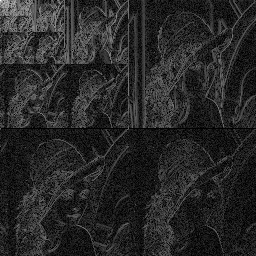
\includegraphics[height=0.25\textwidth]{../images/lenna_d2_before}
		&	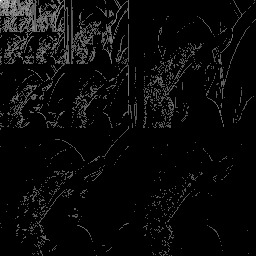
\includegraphics[height=0.25\textwidth]{../images/lenna_d2_after}
		&	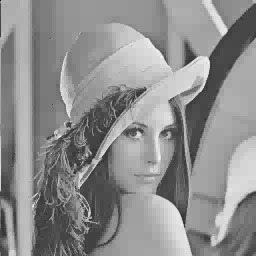
\includegraphics[height=0.25\textwidth]{../images/lenna_d2_final} \\
			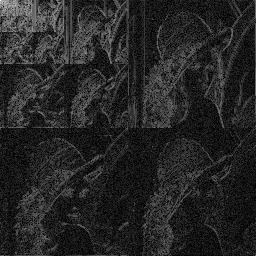
\includegraphics[height=0.25\textwidth]{../images/lenna_d4_before}
		&	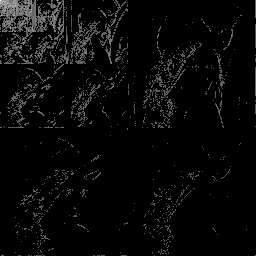
\includegraphics[height=0.25\textwidth]{../images/lenna_d4_after}
		&	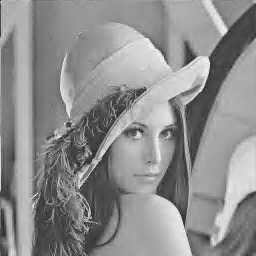
\includegraphics[height=0.25\textwidth]{../images/lenna_d4_final} \\
			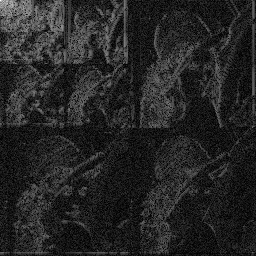
\includegraphics[height=0.25\textwidth]{../images/lenna_d10_before}
		&	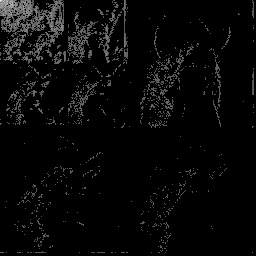
\includegraphics[height=0.25\textwidth]{../images/lenna_d10_after}
		&	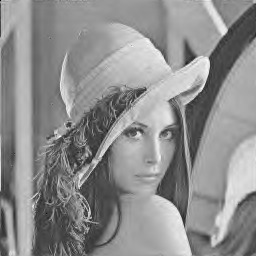
\includegraphics[height=0.25\textwidth]{../images/lenna_d10_final} \\
			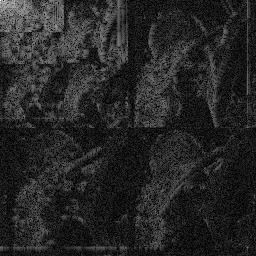
\includegraphics[height=0.25\textwidth]{../images/lenna_d22_before}
		&	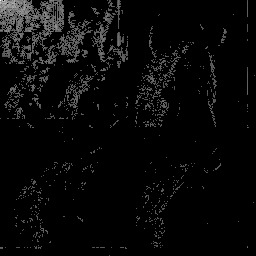
\includegraphics[height=0.25\textwidth]{../images/lenna_d22_after}
		&	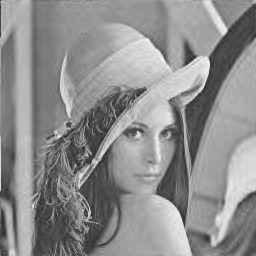
\includegraphics[height=0.25\textwidth]{../images/lenna_d22_final} \\
	\end{tabular} \\
	\caption{By row the Haar, Daubechies-4, Daubechies-10, and Daubechies-22 wavelets were used 
					 respectively. The first
					 column shows the un-modified coefficients.  The second column shows the minimum number
					 of coefficients required to maintain a Mean Square Error of 40.
					 The last column shows the reconstructed(lossy) image.}
\end{figure}

\vfill

\begin{figure}[hbt]
	\centering
	\label{fig:lenna_zeros}
		\includegraphics[angle=-90,width=0.65\textwidth]{../results/graphs/lenna_zeros}
	\caption{Percentage of coefficients in {\bf lenna} with a value of zero. Uses multiple lengths of the Daubechies Wavelet. }
\end{figure}
\begin{figure}[hbt]
	\centering
	\label{fig:lenna_stats}
		\includegraphics[angle=-90,width=0.65\textwidth]{../results/graphs/lenna_results.pdf}
	\caption{Minimum coefficients in {\bf lenna} required to reconstruct with the desired Mean Square Error. Uses multiple lengths of the Daubechies Wavelet. }
\end{figure}

%\vfill

%~%\vfill

%\vfill

%~%\vfill

\begin{figure}[hbt]
	\centering
	\label{fig:boat_imgs}
	\begin{tabular}{ S @{} S @{} S }
		\centering
		& 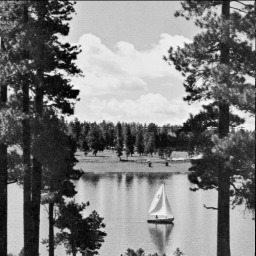
\includegraphics[height=0.25\textwidth]{../images/boat} & \\
			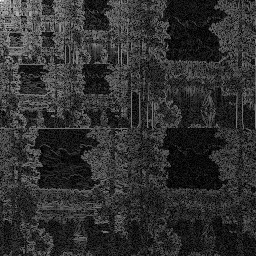
\includegraphics[height=0.25\textwidth]{../images/boat_d2_before}
		&	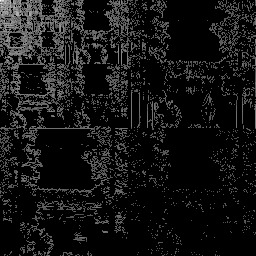
\includegraphics[height=0.25\textwidth]{../images/boat_d2_after}
		&	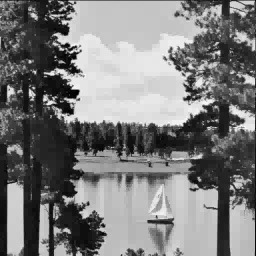
\includegraphics[height=0.25\textwidth]{../images/boat_d2_final} \\
			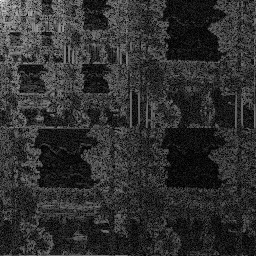
\includegraphics[height=0.25\textwidth]{../images/boat_d4_before}
		&	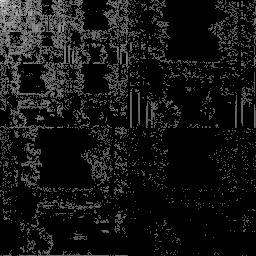
\includegraphics[height=0.25\textwidth]{../images/boat_d4_after}
		&	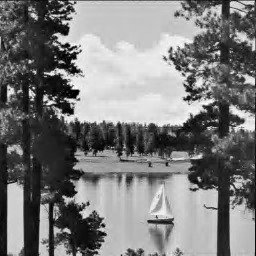
\includegraphics[height=0.25\textwidth]{../images/boat_d4_final} \\
			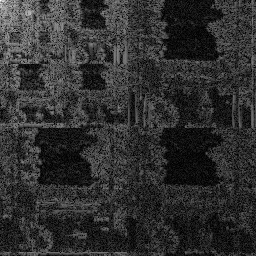
\includegraphics[height=0.25\textwidth]{../images/boat_d10_before}
		&	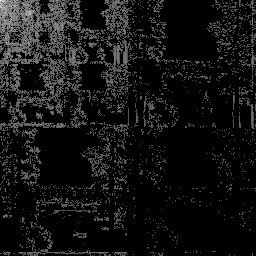
\includegraphics[height=0.25\textwidth]{../images/boat_d10_after}
		&	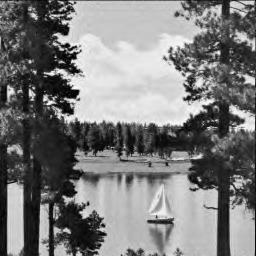
\includegraphics[height=0.25\textwidth]{../images/boat_d10_final} \\
			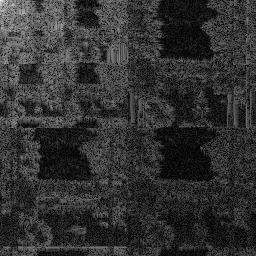
\includegraphics[height=0.25\textwidth]{../images/boat_d22_before}
		&	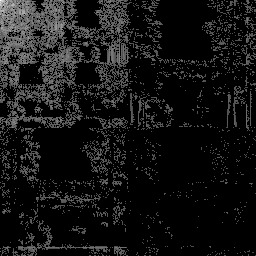
\includegraphics[height=0.25\textwidth]{../images/boat_d22_after}
		&	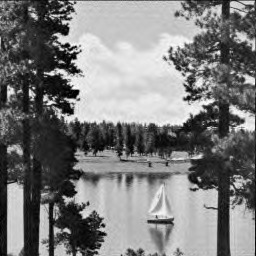
\includegraphics[height=0.25\textwidth]{../images/boat_d22_final} \\
	\end{tabular} \\
	\caption{By row the Haar, Daubechies-4, Daubechies-10, and Daubechies-22 wavelets were used 
					 respectively. The first
					 column shows the un-modified coefficients.  The second column shows the minimum number
					 of coefficients required to maintain a Mean Square Error of 40.
					 The last column shows the reconstructed(lossy) image.}
\end{figure}

%\vfill
\begin{figure}[hbt]
	\centering
	\label{fig:boat_zeros}
		\includegraphics[angle=-90,width=0.65\textwidth]{../results/graphs/boat_zeros}
	\caption{Percentage of coefficients in {\bf boat} with a value of zero. Uses multiple lengths of the Daubechies Wavelet. }
\end{figure}
\begin{figure}[hbt]
	\centering
	\label{fig:boat_stats}
		\includegraphics[angle=-90,width=0.65\textwidth]{../results/graphs/boat_results.pdf}
	\caption{Minimum coefficients in {\bf boat} required to reconstruct with the desired Mean Square Error. Uses multiple lengths of the Daubechies Wavelet. }
\end{figure}


%~%\vfill

%\vfill

%~%\vfill

\begin{figure}[hbt]
	\centering
	\label{fig:f_16_imgs}
	\begin{tabular}{ S @{} S @{} S }
		\centering
		& 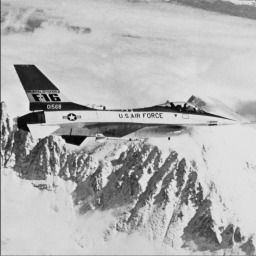
\includegraphics[height=0.25\textwidth]{../images/f_16} & \\
			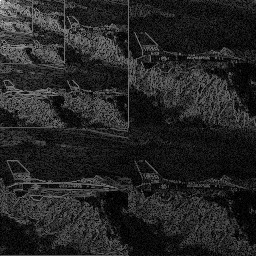
\includegraphics[height=0.25\textwidth]{../images/f_16_d2_before}
		&	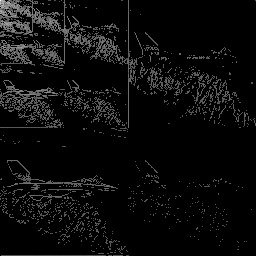
\includegraphics[height=0.25\textwidth]{../images/f_16_d2_after}
		&	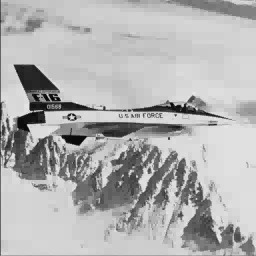
\includegraphics[height=0.25\textwidth]{../images/f_16_d2_final} \\
			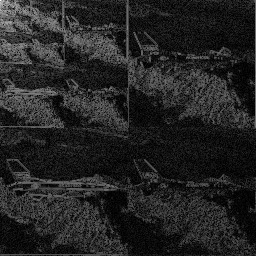
\includegraphics[height=0.25\textwidth]{../images/f_16_d4_before}
		&	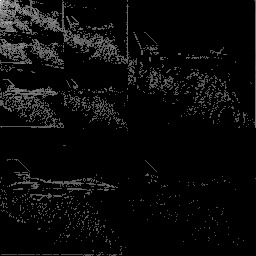
\includegraphics[height=0.25\textwidth]{../images/f_16_d4_after}
		&	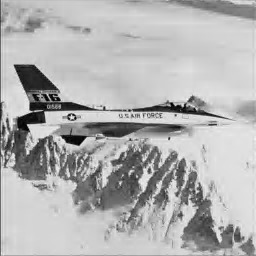
\includegraphics[height=0.25\textwidth]{../images/f_16_d4_final} \\
			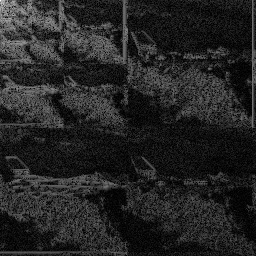
\includegraphics[height=0.25\textwidth]{../images/f_16_d10_before}
		&	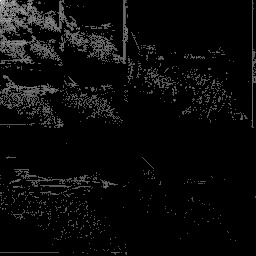
\includegraphics[height=0.25\textwidth]{../images/f_16_d10_after}
		&	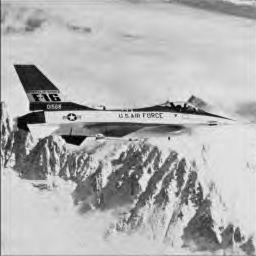
\includegraphics[height=0.25\textwidth]{../images/f_16_d10_final} \\
			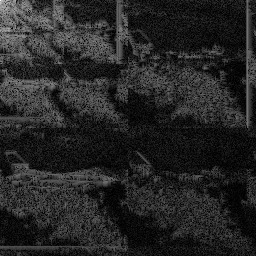
\includegraphics[height=0.25\textwidth]{../images/f_16_d22_before}
		&	\includegraphics[height=0.25\textwidth]{../images/f_16_d22_after}
		&	\includegraphics[height=0.25\textwidth]{../images/f_16_d22_final} \\
	\end{tabular} \\
	\caption{By row the Haar, Daubechies-4, Daubechies-10, and Daubechies-22 wavelets were used 
					 respectively. The first
					 column shows the un-modified coefficients.  The second column shows the minimum number
					 of coefficients required to maintain a Mean Square Error of 40.
					 The last column shows the reconstructed(lossy) image.}
\end{figure}

%\vfill

\begin{figure}[hbt]
	\centering
	\label{fig:f_16_zeros}
		\includegraphics[angle=-90,width=0.65\textwidth]{../results/graphs/f_16_zeros}
	\caption{Percentage of coefficients in {\bf f\_16} with a value of zero. Uses multiple lengths of the Daubechies Wavelet. }
\end{figure}
\begin{figure}[hbt]
	\centering
	\label{fig:f_16_stats}
		\includegraphics[angle=-90,width=0.65\textwidth]{../results/graphs/f_16_results.pdf}
	\caption{Minimum coefficients in {\bf f\_16} required to reconstruct with the desired Mean Square Error. Uses multiple lengths of the Daubechies Wavelet. }
\end{figure}

%~%\vfill

%\vfill

%~%\vfill

\begin{figure}[hbt]
	\centering
	\label{fig:peppers_imgs}
	\begin{tabular}{ S @{} S @{} S }
		\centering
		& \includegraphics[height=0.25\textwidth]{../images/peppers} & \\
			\includegraphics[height=0.25\textwidth]{../images/peppers_d2_before}
		&	\includegraphics[height=0.25\textwidth]{../images/peppers_d2_after}
		&	\includegraphics[height=0.25\textwidth]{../images/peppers_d2_final} \\
			\includegraphics[height=0.25\textwidth]{../images/peppers_d4_before}
		&	\includegraphics[height=0.25\textwidth]{../images/peppers_d4_after}
		&	\includegraphics[height=0.25\textwidth]{../images/peppers_d4_final} \\
			\includegraphics[height=0.25\textwidth]{../images/peppers_d10_before}
		&	\includegraphics[height=0.25\textwidth]{../images/peppers_d10_after}
		&	\includegraphics[height=0.25\textwidth]{../images/peppers_d10_final} \\
			\includegraphics[height=0.25\textwidth]{../images/peppers_d22_before}
		&	\includegraphics[height=0.25\textwidth]{../images/peppers_d22_after}
		&	\includegraphics[height=0.25\textwidth]{../images/peppers_d22_final} \\
	\end{tabular} \\
	\caption{By row the Haar, Daubechies-4, Daubechies-10, and Daubechies-22 wavelets were used 
					 respectively. The first
					 column shows the un-modified coefficients.  The second column shows the minimum number
					 of coefficients required to maintain a Mean Square Error of 40.
					 The last column shows the reconstructed(lossy) image.}
\end{figure}

%\vfill
\begin{figure}[hbt]
	\centering
	\label{fig:peppers_zeros}
		\includegraphics[angle=-90,width=0.65\textwidth]{../results/graphs/peppers_zeros}
	\caption{Percentage of coefficients in {\bf peppers} with a value of zero. Uses multiple lengths of the Daubechies Wavelet. }
\end{figure}
\begin{figure}[hbt]
	\centering
	\label{fig:peppers_stats}
		\includegraphics[angle=-90,width=0.65\textwidth]{../results/graphs/peppers_results.pdf}
	\caption{Minimum coefficients in {\bf peppers} required to reconstruct with the desired Mean Square Error. Uses multiple lengths of the Daubechies Wavelet. }
\end{figure}


%~%\vfill

%\vfill

%~%\vfill

\begin{figure}[hbt]
	\centering
	\label{fig:tools_imgs}
	\begin{tabular}{ S @{} S @{} S }
		\centering
		& \includegraphics[height=0.25\textwidth]{../images/tools} & \\
			\includegraphics[height=0.25\textwidth]{../images/tools_d2_before}
		&	\includegraphics[height=0.25\textwidth]{../images/tools_d2_after}
		&	\includegraphics[height=0.25\textwidth]{../images/tools_d2_final} \\
			\includegraphics[height=0.25\textwidth]{../images/tools_d4_before}
		&	\includegraphics[height=0.25\textwidth]{../images/tools_d4_after}
		&	\includegraphics[height=0.25\textwidth]{../images/tools_d4_final} \\
			\includegraphics[height=0.25\textwidth]{../images/tools_d10_before}
		&	\includegraphics[height=0.25\textwidth]{../images/tools_d10_after}
		&	\includegraphics[height=0.25\textwidth]{../images/tools_d10_final} \\
			\includegraphics[height=0.25\textwidth]{../images/tools_d22_before}
		&	\includegraphics[height=0.25\textwidth]{../images/tools_d22_after}
		&	\includegraphics[height=0.25\textwidth]{../images/tools_d22_final} \\
	\end{tabular} \\
	\caption{By row the Haar, Daubechies-4, Daubechies-10, and Daubechies-22 wavelets were used 
					 respectively. The first
					 column shows the un-modified coefficients.  The second column shows the minimum number
					 of coefficients required to maintain a Mean Square Error of 40.
					 The last column shows the reconstructed(lossy) image.}
\end{figure}

%\vfill

\begin{figure}[hbt]
	\centering
	\label{fig:tools_zeros}
		\includegraphics[angle=-90,width=0.65\textwidth]{../results/graphs/tools_zeros}
	\caption{Percentage of coefficients in {\bf tools} with a value of zero. Uses multiple lengths of the Daubechies Wavelet.  Please note that this percentage is based on the number of pixels in the original image.  Because the FFT requires the image be padded with zeros to a power of 2, more non-zero coefficients exist than pixels in the original image.  }
\end{figure}
\begin{figure}[hbt]
	\centering
	\label{fig:tools_stats}
		\includegraphics[angle=-90,width=0.65\textwidth]{../results/graphs/tools_results.pdf}
	\caption{Minimum coefficients in {\bf tools} required to reconstruct with the desired Mean Square Error. Uses multiple lengths of the Daubechies Wavelet. }
\end{figure}

%~%\vfill

%\vfill

%~%\vfill

\begin{figure}[hbt]
	\centering
	\label{fig:wheel_imgs}
	\begin{tabular}{ S @{} S @{} S }
		\centering
		& \includegraphics[height=0.25\textwidth]{../images/wheel} & \\
			\includegraphics[height=0.25\textwidth]{../images/wheel_d2_before}
		&	\includegraphics[height=0.25\textwidth]{../images/wheel_d2_after}
		&	\includegraphics[height=0.25\textwidth]{../images/wheel_d2_final} \\
			\includegraphics[height=0.25\textwidth]{../images/wheel_d4_before}
		&	\includegraphics[height=0.25\textwidth]{../images/wheel_d4_after}
		&	\includegraphics[height=0.25\textwidth]{../images/wheel_d4_final} \\
			\includegraphics[height=0.25\textwidth]{../images/wheel_d10_before}
		&	\includegraphics[height=0.25\textwidth]{../images/wheel_d10_after}
		&	\includegraphics[height=0.25\textwidth]{../images/wheel_d10_final} \\
			\includegraphics[height=0.25\textwidth]{../images/wheel_d22_before}
		&	\includegraphics[height=0.25\textwidth]{../images/wheel_d22_after}
		&	\includegraphics[height=0.25\textwidth]{../images/wheel_d22_final} \\
	\end{tabular} \\
	\caption{By row the Haar, Daubechies-4, Daubechies-10, and Daubechies-22 wavelets were used 
					 respectively. The first
					 column shows the un-modified coefficients.  The second column shows the minimum number
					 of coefficients required to maintain a Mean Square Error of 40.
					 The last column shows the reconstructed(lossy) image.}
\end{figure}

~\vfill
\FloatBarrier

\begin{figure}[hbt]
	\centering
	\label{fig:wheel_zeros}
		\includegraphics[angle=-90,width=0.65\textwidth]{../results/graphs/wheel_zeros}
	\caption{Percentage of coefficients in {\bf wheel} with a value of zero. Uses multiple lengths of the Daubechies Wavelet. }
\end{figure}
\begin{figure}[hbt]
	\centering
	\label{fig:wheel_stats}
		\includegraphics[angle=-90,width=0.65\textwidth]{../results/graphs/wheel_results.pdf}
	\caption{Minimum coefficients in {\bf wheel} required to reconstruct with the desired Mean Square Error. Uses multiple lengths of the Daubechies Wavelet. }
\end{figure}

\vfill

\begin{figure}[hbt]
	\centering
	\label{fig:konye_imgs}
	\begin{tabular}{ S @{} S @{} S }
		\centering
		& \includegraphics[height=0.25\textwidth]{../images/konye} & \\
			\includegraphics[height=0.25\textwidth]{../images/konye_d2_before}
		&	\includegraphics[height=0.25\textwidth]{../images/konye_d2_after}
		&	\includegraphics[height=0.25\textwidth]{../images/konye_d2_final} \\
			\includegraphics[height=0.25\textwidth]{../images/konye_d4_before}
		&	\includegraphics[height=0.25\textwidth]{../images/konye_d4_after}
		&	\includegraphics[height=0.25\textwidth]{../images/konye_d4_final} \\
			\includegraphics[height=0.25\textwidth]{../images/konye_d10_before}
		&	\includegraphics[height=0.25\textwidth]{../images/konye_d10_after}
		&	\includegraphics[height=0.25\textwidth]{../images/konye_d10_final} \\
			\includegraphics[height=0.25\textwidth]{../images/konye_d22_before}
		&	\includegraphics[height=0.25\textwidth]{../images/konye_d22_after}
		&	\includegraphics[height=0.25\textwidth]{../images/konye_d22_final} \\
	\end{tabular} \\
	\caption{By row the Haar, Daubechies-4, Daubechies-10, and Daubechies-22 wavelets were used 
					 respectively. The first
					 column shows the un-modified coefficients.  The second column shows the minimum number
					 of coefficients required to maintain a Mean Square Error of 40.
					 The last column shows the reconstructed(lossy) image.}
\end{figure}

\begin{figure}[hbt]
	\centering
	\label{fig:konye_zeros}
		\includegraphics[angle=-90,width=0.65\textwidth]{../results/graphs/konye_zeros}
	\caption{Percentage of coefficients in {\bf konye} with a value of zero. Uses multiple lengths of the Daubechies Wavelet. }
\end{figure}
\begin{figure}[hbt]
	\centering
	\label{fig:konye_stats}
		\includegraphics[angle=-90,width=0.65\textwidth]{../results/graphs/konye_results.pdf}
	\caption{Minimum coefficients in {\bf konye} required to reconstruct with the desired Mean Square Error. Uses multiple lengths of the Daubechies Wavelet. }
\end{figure}

\begin{figure}[hbt]
	\centering
	\label{fig:gradient_imgs}
	\begin{tabular}{ S @{} S @{} S }
		\centering
		& \includegraphics[height=0.25\textwidth]{../images/gradient} & \\
			\includegraphics[height=0.25\textwidth]{../images/gradient_d2_before}
		&	\includegraphics[height=0.25\textwidth]{../images/gradient_d2_after}
		&	\includegraphics[height=0.25\textwidth]{../images/gradient_d2_final} \\
			\includegraphics[height=0.25\textwidth]{../images/gradient_d4_before}
		&	\includegraphics[height=0.25\textwidth]{../images/gradient_d4_after}
		&	\includegraphics[height=0.25\textwidth]{../images/gradient_d4_final} \\
			\includegraphics[height=0.25\textwidth]{../images/gradient_d10_before}
		&	\includegraphics[height=0.25\textwidth]{../images/gradient_d10_after}
		&	\includegraphics[height=0.25\textwidth]{../images/gradient_d10_final} \\
			\includegraphics[height=0.25\textwidth]{../images/gradient_d22_before}
		&	\includegraphics[height=0.25\textwidth]{../images/gradient_d22_after}
		&	\includegraphics[height=0.25\textwidth]{../images/gradient_d22_final} \\
	\end{tabular} \\
	\caption{By row the Haar, Daubechies-4, Daubechies-10, and Daubechies-22 wavelets were used 
					 respectively. The first
					 column shows the un-modified coefficients.  The second column shows the minimum number
					 of coefficients required to maintain a Mean Square Error of 40.
					 The last column shows the reconstructed(lossy) image.}
\end{figure}

\begin{figure}[hbt]
	\centering
	\label{fig:gradient_zeros}
		\includegraphics[angle=-90,width=0.65\textwidth]{../results/graphs/gradient_zeros}
	\caption{Percentage of coefficients in {\bf gradient} with a value of zero. Uses multiple lengths of the Daubechies Wavelet. }
\end{figure}
\begin{figure}[hbt]
	\centering
	\label{fig:gradient_stats}
		\includegraphics[angle=-90,width=0.65\textwidth]{../results/graphs/gradient_results.pdf}
	\caption{Minimum coefficients in {\bf gradient} required to reconstruct with the desired Mean Square Error. Uses multiple lengths of the Daubechies Wavelet. }
\end{figure}

%\vfill
